\section{Ввод временных координат}
\begin{enumerate}[\thesection .1]
	\item Для получения "временных координат" торговой точки, необходимо находясь 
	(рис.\ref{pic:pic9_1})
	\begin{figure}[!h]
		\begin{floatrow}
			\ffigbox{\caption{Выбор типа синхронизации}\label{pic:pic9_1}}%
			{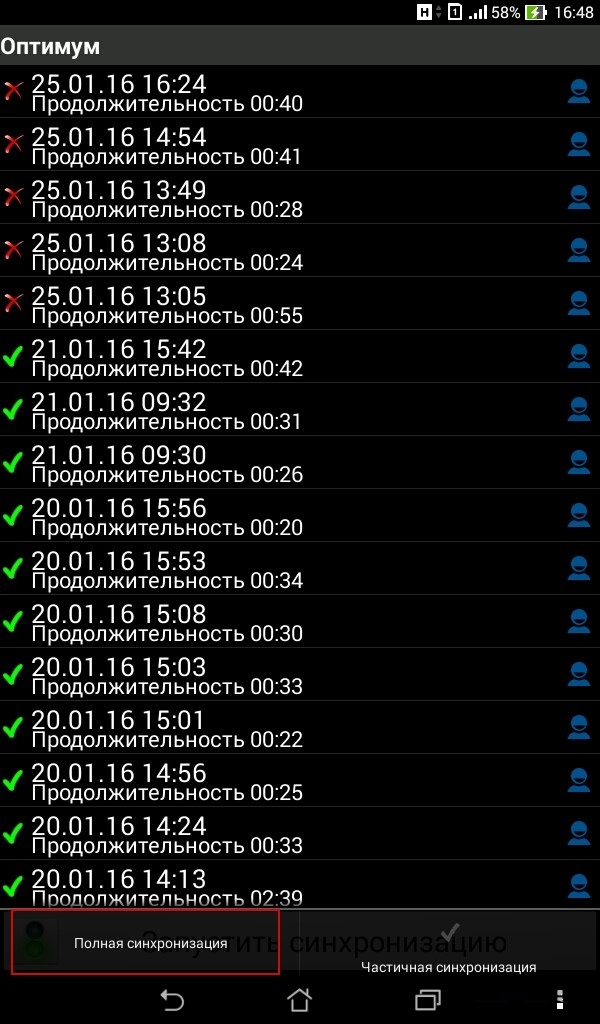
\includegraphics[width=0.8\linewidth]{scr9_1.jpg}}
		\end{floatrow}
	\end{figure}
	Нужно отметить тип <<Полная синхронизация>>, а затем запустить синхронизацию
\end{enumerate}	